\newcommand{\psd}[1]{{\small\sffamily{\color{blue!60}#1}}}

\section{Introduction}

This tutorial is concerned with a non-linear problem of the incremental
analysis of an elasto-plastic Von-Mises material. A two-dimensional test
(in \(x-y\)) will be considered. The problem of interest is a quarter of
a cylinder (with external radius \(R_e\) and internal radius \(R_i\))
\cref{bar-sd}. Boundary conditions correspond to symmetry conditions on
the bottom horizontal \(y=0\) and left vertical borders \(x=0\) (resp.
numbered 1 and 3 as mesh labels). Loading consists of a uniform pressure
(traction boundary) on the internal boundary (numbered 4 as mesh label).
Load (pressure) \(q\) will be progressively increased from 0 to
\(q_{\text{lim}}=\frac{2}{\sqrt3}\sigma_0\text{log}(\frac{R_e}{R_i})\)
which is the analytical collapse load for a perfectly-plastic material
(no hardening):

\begin{figure}[h!]
\centering
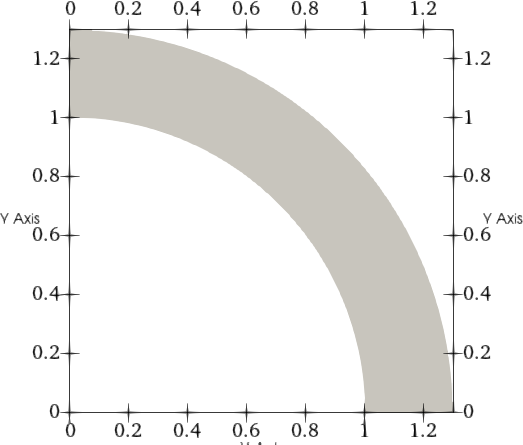
\includegraphics[width=0.3\textwidth]{./Images/nl-arc.png}
\caption{Domain of the non-linear problem. \label{bar-sd}}
\end{figure}

The material is represented by an isotropic elasto-plastic von Mises
yield condition of uniaxial strength \(\sigma_0\) and with isotropic
hardening of modulus \(H\). The yield condition is thus given by:

\[f(\sigma)=\sqrt{\frac{3}{2}s:s}-\sigma_0-Hp\le0\]

where \(p\) is the cumulated equivalent plastic strain and \(s\)
denoting the deviatoric elastic stress
\(s = \text{dev} \sigma_{\text{elas}}\). The hardening modulus can also
be related to a tangent elastic modulus \(E_t=\frac{EH}{E+H}\).

To compute the structures response an iterative predictor-corrector
return mapping algorithm embedded in a Newton-Raphson global loop for
restoring equilibrium is used. Due to the simple expression of the von
Mises criterion, the return mapping procedure is completely analytical
(with linear isotropic hardening). We point out that the two-dimensional
nature of the problem will be impose keeping track of the out-of-plane
\(\varepsilon^p_{zz}\) plastic strain and dealing with representations
of stress/strain states including the \(zz\) component.

The displacement field evolution during the cylinder expansion will look
like this the one presented in \cref{bar-sd}:

\begin{figure}[h!]
\centering
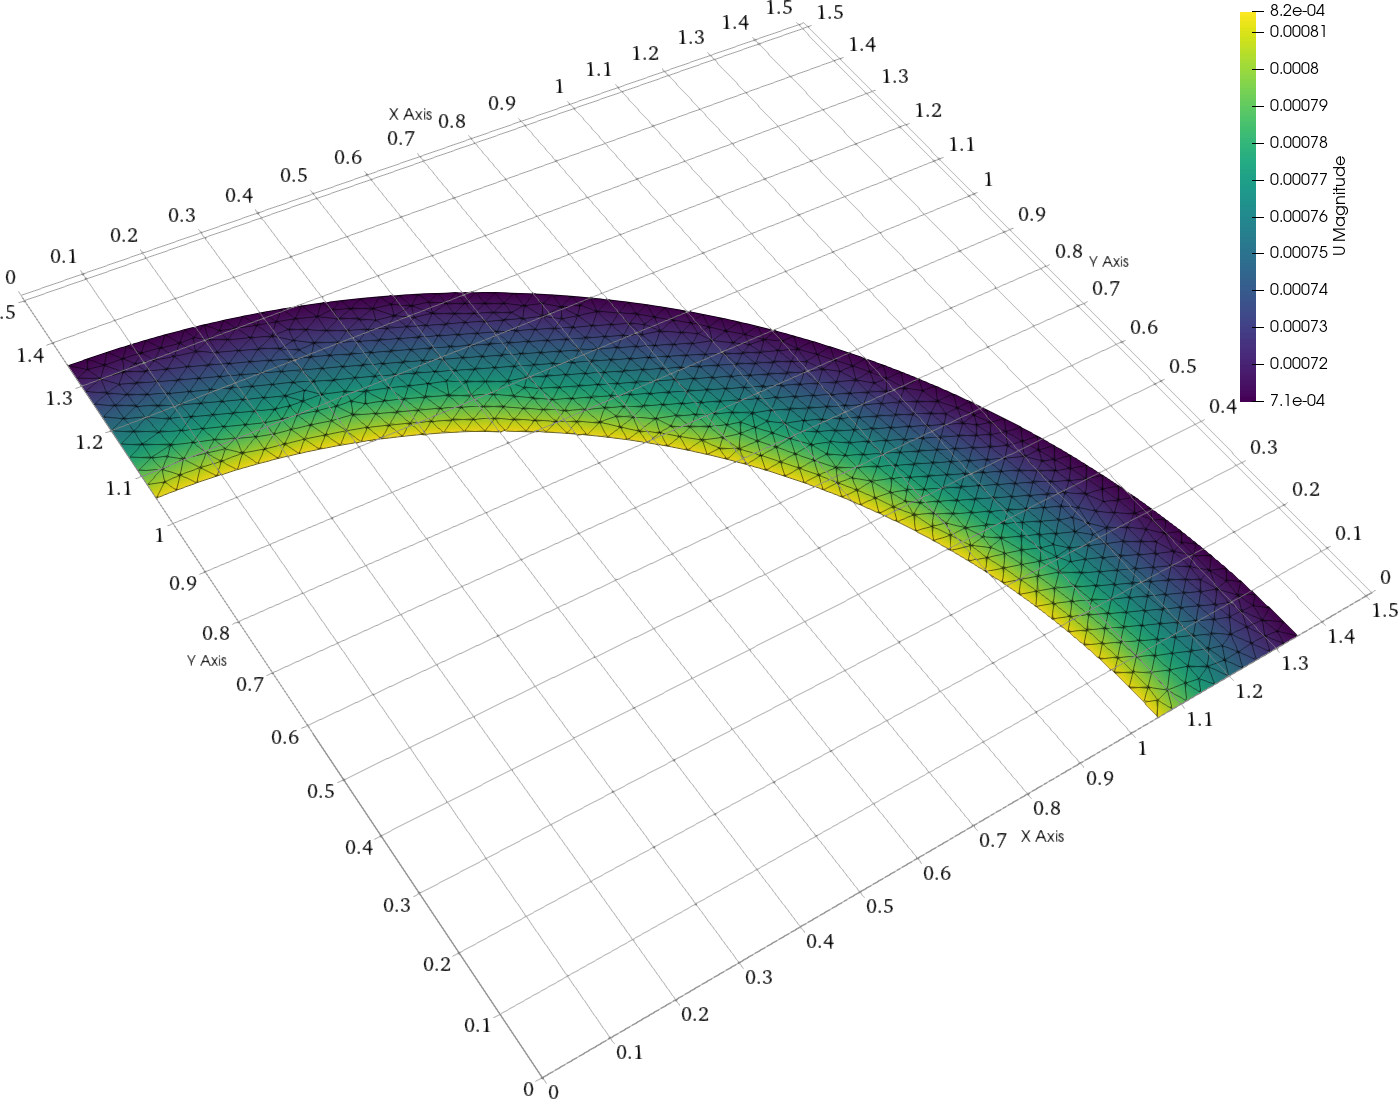
\includegraphics[width=0.3\textwidth]{./Images/nl-ep-t0.png}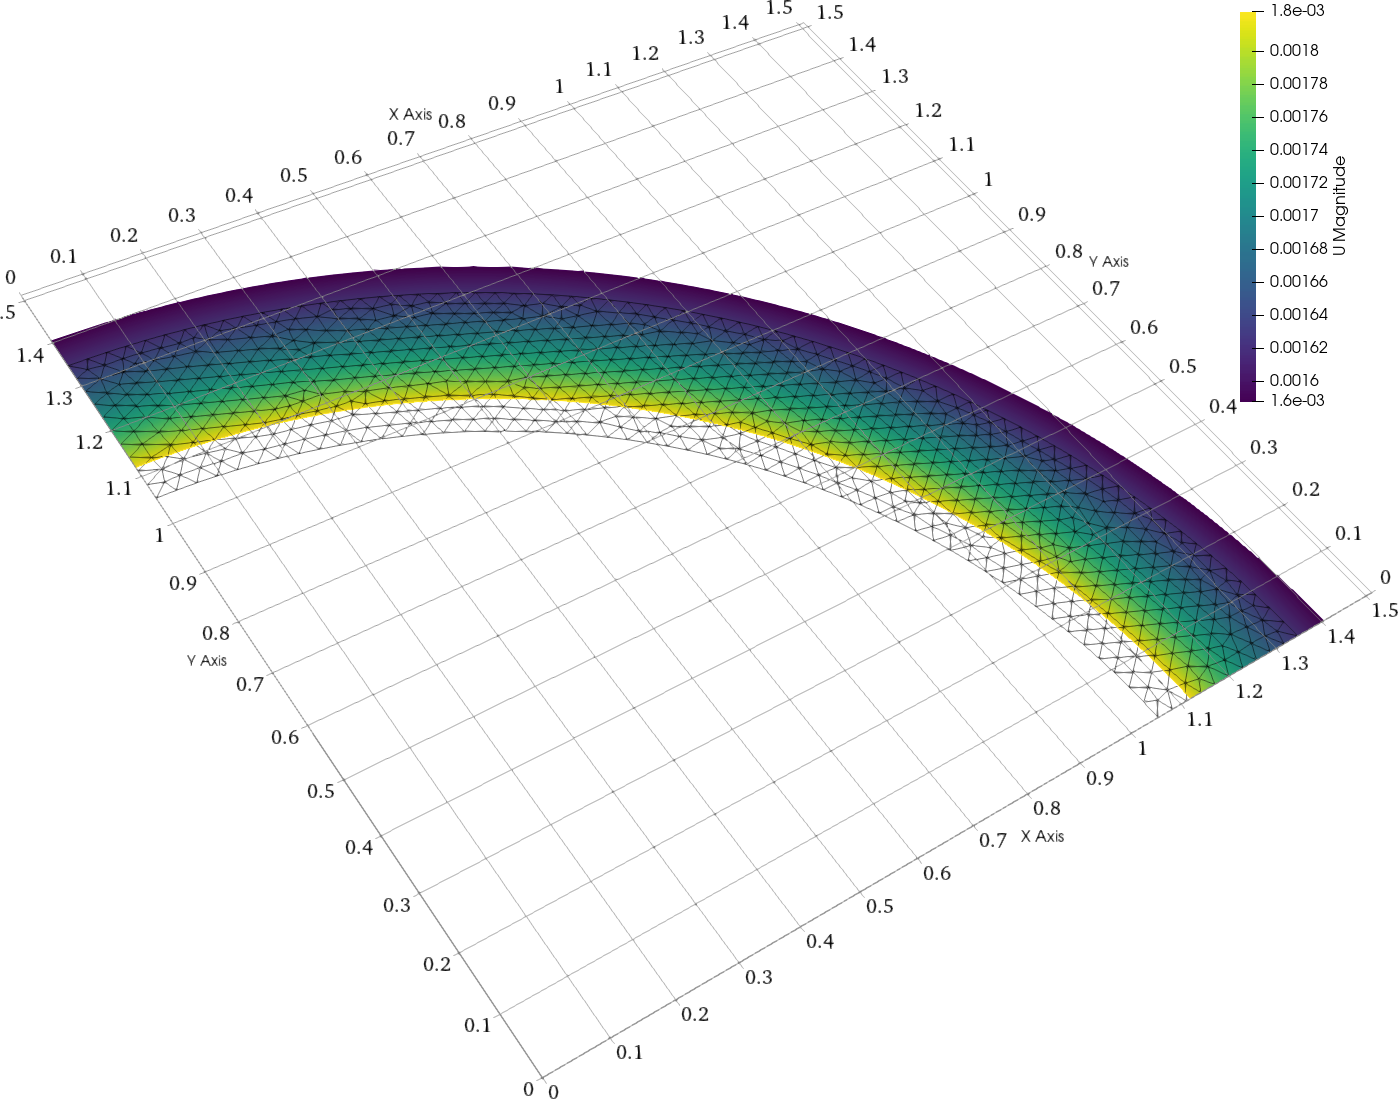
\includegraphics[width=0.3\textwidth]{./Images/nl-ep-t4.png}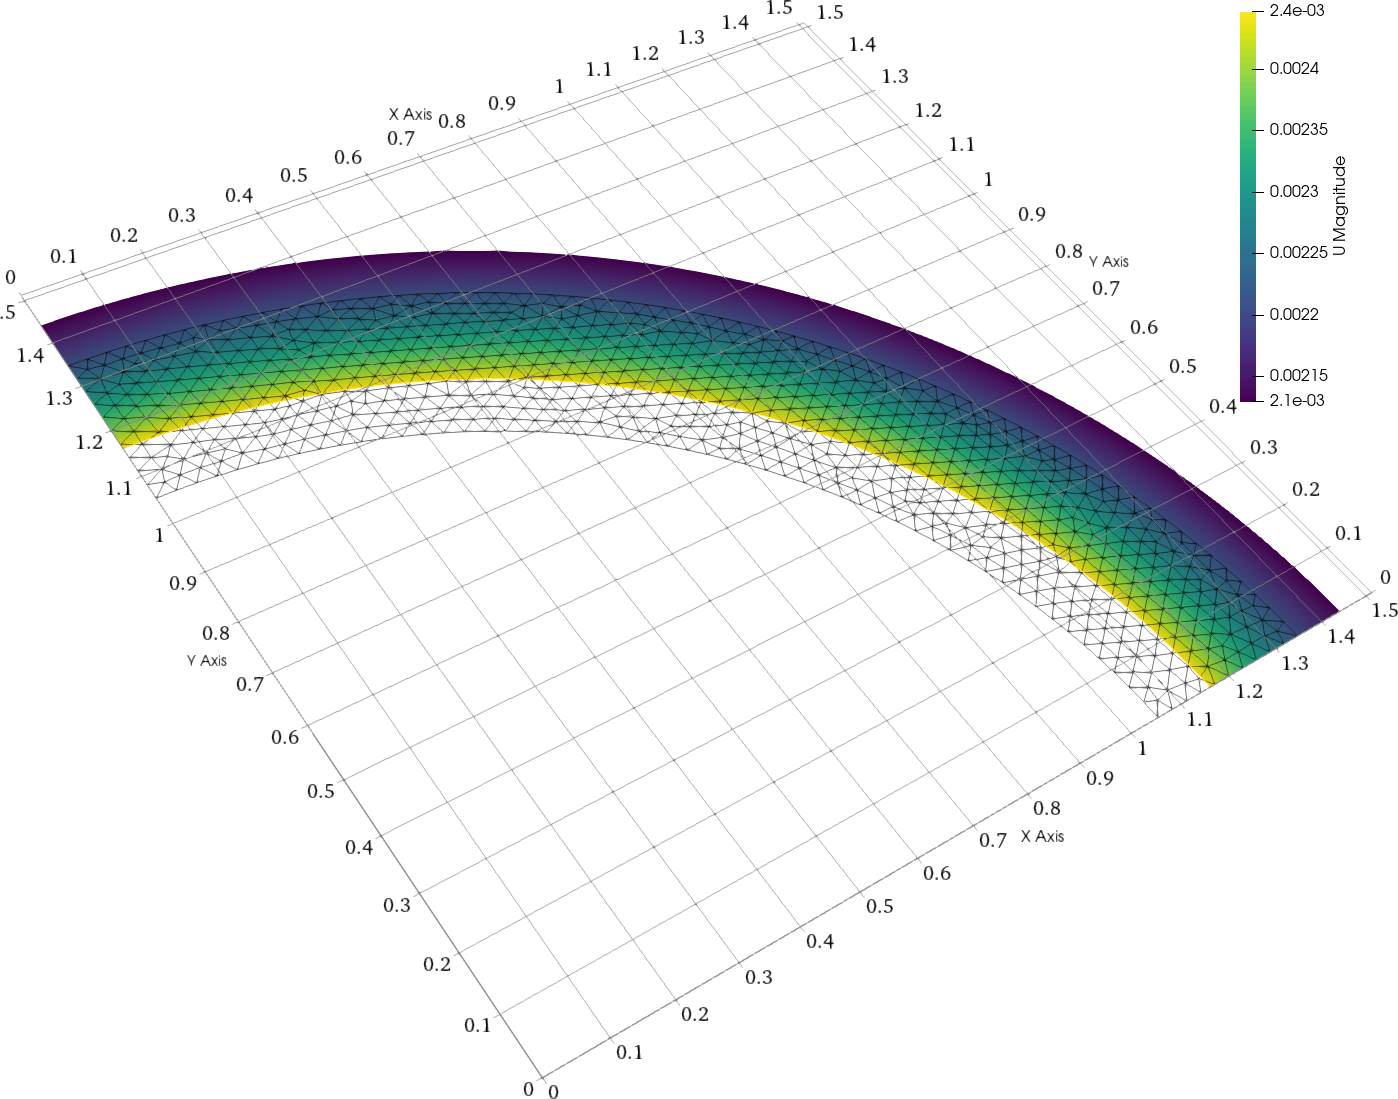
\includegraphics[width=0.3\textwidth]{./Images/nl-ep-t8.png}\\
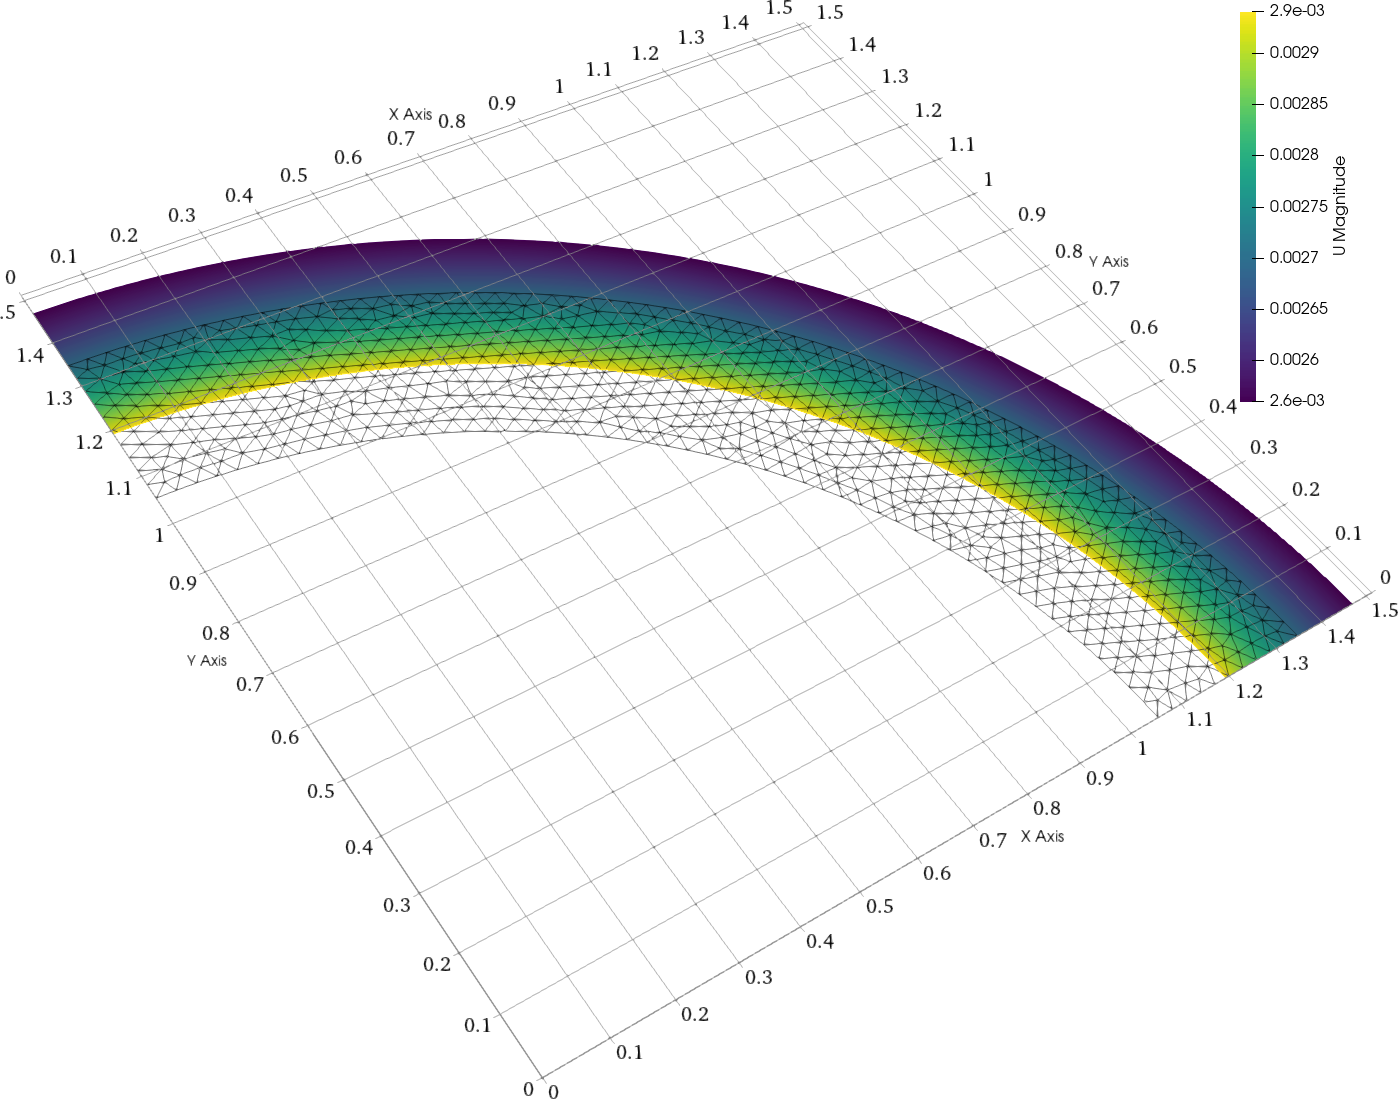
\includegraphics[width=0.3\textwidth]{./Images/nl-ep-t12.png}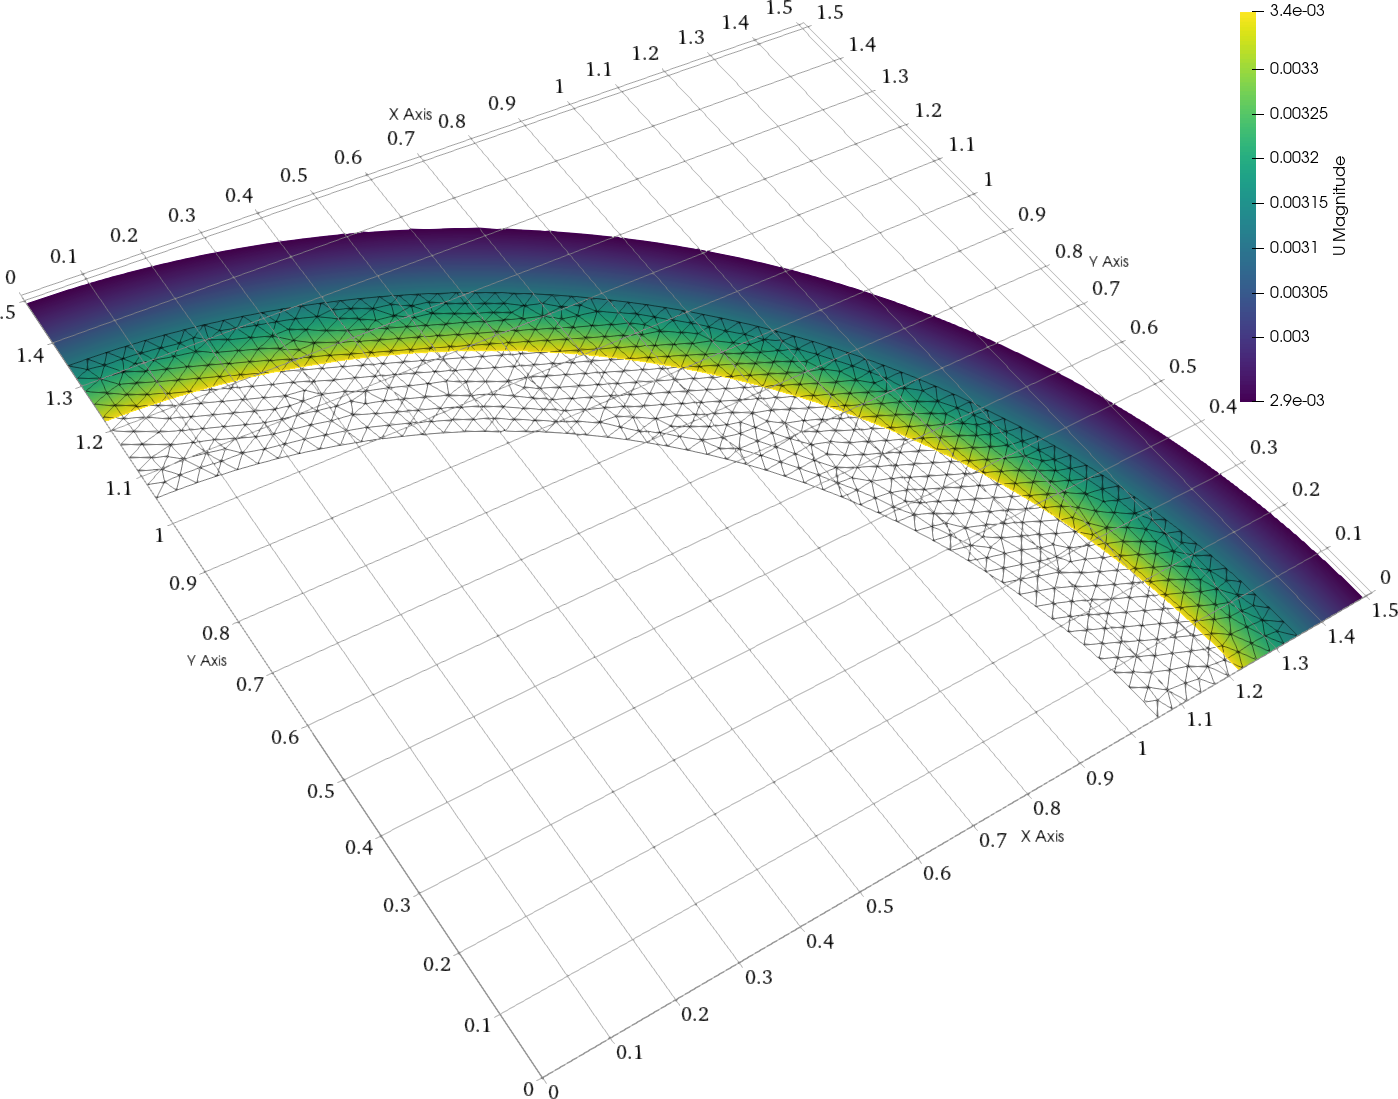
\includegraphics[width=0.3\textwidth]{./Images/nl-ep-t16.png}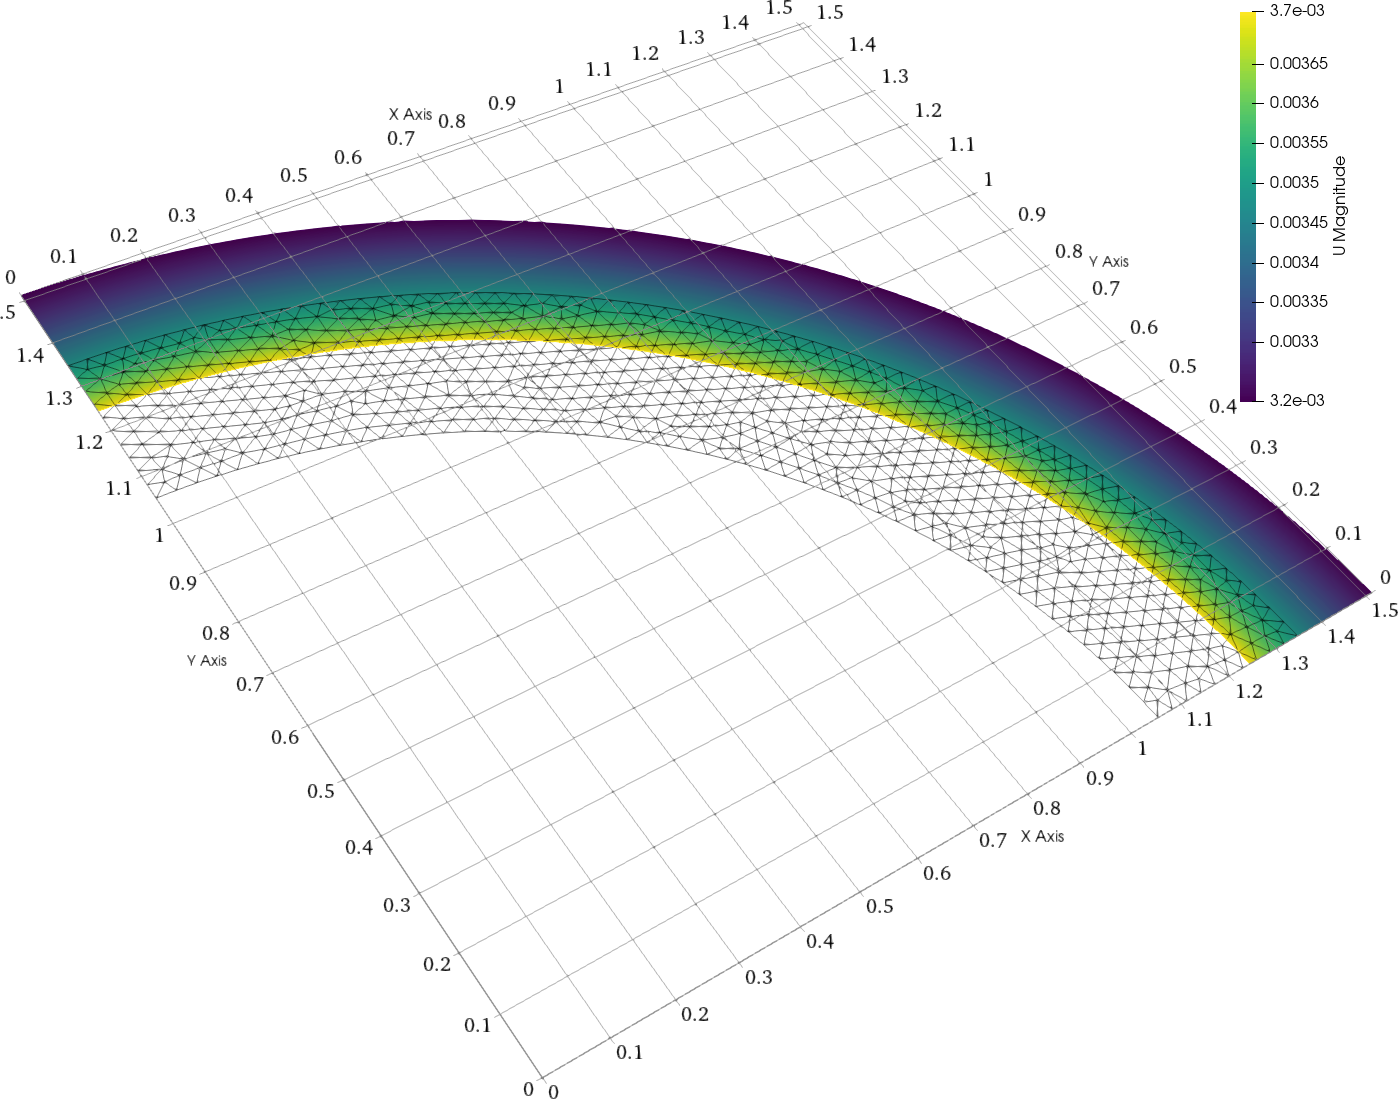
\includegraphics[width=0.3\textwidth]{./Images/nl-ep-t19.png}
\caption{Warped displacement field evolution - from top left $t_0,t_4,t_8,t_{12},t_{16},t_{19}$. \label{bar-sd}}
\end{figure}

The return mapping procedure consists in finding a new stress
\(\sigma_{n+1}\) and internal variable \(p_{n+1}\) state verifying the
current plasticity condition from a previous stress \(\sigma_n\) and
internal variable \(p_{n}\) state and an increment of total deformation
\(\Delta \varepsilon\). All this is handled by MFront, where MFront
requests PSD for the previous \(n\) time-step strains \(\varepsilon_n\).
In order to use a Newton-Raphson procedure to resolve global
equilibrium, we also need to derive the algorithmic consistent tangent
matrix which is also given by MFront.

Within MFront an elastic trial stress
\(\sigma_{\text{elas}} = \sigma_{n} + \mathbf{M}\Delta \varepsilon\) is
first computed. Then the plasticity criterion is then evaluated with the
previous plastic strain
\(f_{\text{elas}}=\sigma_{\text{elas}}^{\text{eq}} - \sigma_0 - Hp_n\),
where \(\sigma_{\text{elas}}^{\text{eq}}=\sqrt{\frac{3}{2}s:s}\).
Consequently, if \(f_{\text{elas}} \le 0\) no plasticity occurs during
this time increment and \(\Delta \varepsilon^p = \Delta p =0\).
Otherwise if \(f_{\text{elas}} > 0\), plasticity occurs and the
increment of plastic strain is given by
\[\Delta p = \frac{f_{\text{elas}}}{3\mu + H}\]

The final stress state is corrected by the plastic strain as follows

\[\sigma_{n+1} = \sigma_{\text{elas}} - \beta s \quad \text{with} \quad \beta=\frac{3\mu}{\sigma_{\text{elas}}^{\text{eq}}}\Delta p\]

\section{Procedure to simulate in PSD}

\subsection{Step 1: Preprocessing}

First step in a PSD simulation is PSD preprocessing, at this step you
tell PSD what kind of physics, boundary conditions, approximations,
mesh, etc are you expecting to solve. More importantly for this tutorial
we will signify to PSD that MFront has to be used.

In the terminal \psd{cd} to the folder
\psd{/home/PSD-tutorials/elasto-plastic}. Launch \psd{PSD\_PreProcess}
from the terminal, to do so run the following command.

\begin{lstlisting}[style=BashInputStyle]
PSD_PreProcess -problem elasto_plastic -model von_mises -dimension 2 \
-tractionconditions 1  -dirichletconditions 2 -postprocess u -useMfront
\end{lstlisting}

After the \psd{PSD\_PreProcess} runs successfully you should see many
\psd{.edp} files in your current folder.

\textbf{What do the arguments mean ?}

\begin{itemize}
\item \psd{-problem elasto\_plastic} means that we are solving elasto plastic problem;
\item \psd{-model von\_mises} means that we are using Von Mises hypothesis;
\item \psd{-dimension 2} means it is a 2D simulation;
\item \psd{-tractionconditions 1} with applied traction force acting on the domain border (pressure);
\item \psd{-dirichletconditions 2} says we have two Dirichlet border;
\item \psd{-postprocess u} means we would like to have ParaView post processing files.
\item \psd{-useMfront} activates MFront interface for PSD.
\end{itemize}

At this stage the input properties \(E,\nu, \sigma_0, E_t, H\) ,
Geometric parameters (internal/external radius of shell) \(R_i, R_e\),
and limiting pressure \(Q_{\text{lim}}\) can be mentioned in
\psd{ControlParameters.edp}. Some of these properties will be shared
with MFront. Have a look at the below given snippet from the file
\psd{ControlParameters.edp}

\begin{lstlisting}[style=CppStyle]
//============================================================================
//                   ------- Material parameters -------                      
// -------------------------------------------------------------------        
//  E, nu : Modulus of Elasticity and Poisson ratio of the material           
//  sig0  : Yield strength of the material                                    
//  Et    : Tangent modulus of the material                                   
//  H     : Hardening modulus of the material                                 
//  PropertyNames : String of material property names (space seperated)       
//                  that are provided to Mfront.                              
//  PropertyValues : Values of material properties provided to Mfront         
//                                                                            
// -------------------------------------------------------------------        
//  NOTE:     Please note that PropertyNames should be the same as            
//            as in the Elasticity.mfront file                                
// -------------------------------------------------------------------        
//============================================================================
                                                                              
  real E    = 70.e3       ,                                                   
       nu   = 0.3         ,                                                   
       sig0 = 250.        ,                                                   
       Et   = E/100.      ,                                                   
       H    = E*Et/(E-Et) ;                                                   
                                                                              
                                                                              
  real Re   = 1.3         ,  // external radius geometry                      
       Ri   = 1.0         ;  // internal radius geometry                      
                                                                              
                                                                              
  real Qlim = 2./sqrt(3.)*log(Re/Ri)*sig0; //  Limiting pressure 
\end{lstlisting}

We then move on to defining the MFront parameters. We, create variables
that can be exchanged with MFront and inform MFront that we would like
to use IsotropicLinearHardeningPlasticity model with PLAINSTRAIN
hypothesis (since we are in 2D) and the given properties. Have a look at
the below given snippet from the file \psd{ControlParameters.edp}

\begin{lstlisting}[style=CppStyle]
  string    MaterialBehaviour   = "IsotropicLinearHardeningPlasticity";     
  string    MaterialHypothesis  = "PLANESTRAIN";                 
  string    PropertyNames       = "YoungModulus PoissonRatio HardeningSlope YieldStrength";
  real[int] PropertyValues      = [ E, nu , H, sig0 ];
\end{lstlisting}

The algorithmic parameters will be set up next, i.e, we signify the
Newton-Raphsons convergence criteria, Newton-Raphsons maximum
iterations, and number of time steps for quasi-time discretization. Have
a look at the below given snippet from the file
\psd{ControlParameters.edp}

\begin{lstlisting}[style=CppStyle]
//============================================================================
//                   ------- Algorithmic parameters -------                   
// -------------------------------------------------------------------        
//  NrEpsCon : Newton-Raphsons Convergence epsilon                            
//  NrMaxItr : Newton-Raphsons maximum iterations                             
//  TlMaxItr : Number of time steps for quasi-time discretization             
//                                                                            
// -------------------------------------------------------------------        
//  NOTE:     Please note that PropertyNames should be the same as            
//            as in the Elasticity.mfront file                                
// -------------------------------------------------------------------        
//============================================================================
                                                                              
  macro EpsNrCon  ()   1.e-8       //                                         
  macro NrMaxItr  ()   200         //                                         
  macro TlMaxItr  ()   20          // 
\end{lstlisting}

Next we notify PSD about the Dirichlet conditions since two Dirichlet
conditions exists we need to provide info about these in. To provide the
\(y\) constained boundary condition (border of the cylinder on
\(x\)-axis) the variables \psd{Dbc0On 1}, \psd{Dbc0Uy 0.}, which means
for Dirichlet border \psd{1} (\psd{Dbc0On 1}) where \psd{1} is the
constrained in \(y\) direction label of the mesh Dirichlet constrain is
applied \psd{Dbc0Uy 0} i.e., the clamped end condition (for
\(\partial\Omega_{\text{meshLabel==1}}\) \(u_y=0\)). Similarly the
Dirichlet constrain is set on vertical border (border of the cylinder on
\(y\)-axis), where \(\partial\Omega_{\text{meshLabel==3}}\) \(u_x=0\).
Have a look at the below given snippet from the file
\psd{ControlParameters.edp}

\begin{lstlisting}[style=CppStyle]
//============================================================================
//        ------- Dirichlet boundary-condition parameters -------             
// ---------------------------------------------------------------------------
// Dbc       : acronym for Dirichlet boundary condition                       
// Dbc(I)On  : is/are the  surface labels tags (integer list) on to which     
//             Dirichlet boundary conditions is to be applied.                
// Dbc(I)Ux  : is the x component of Dirichlet displacement on the surface    
//             border (I) denoted by label(s) Dbc(I)On in the mesh.           
// -------------------------------------------------------------------------- 
// NOTE: either macro Dbc(I)Ux or Dbc(I)Uy or Dbc(I)Uz should  be commented   
//       or deleted if the user does not wish to apply Dirichlet  condition   
//       on that particular  direction (let it free)                          
//============================================================================
                                                                              
  macro  Dbc0On 1   //                            
  macro  Dbc0Uy 0.  //                                               
  macro  Dbc1On 3   //                            
  macro  Dbc1Ux 0.  // 
\end{lstlisting}

Next we set up the traction (pressure) conditions. Have a look at the
below given snippet from the file \psd{ControlParameters.edp}

\begin{lstlisting}[style=CppStyle]
//============================================================================
// ------- Neumann/traction boundary-condition parameters -------             
// ---------------------------------------------------------------------------
// Tbc       : acronym for traction boundary condition                        
// Tbc(I)On  : is/are the  surface labels tags (integer list) on to which     
//             traction boundary conditions is to be applied.                 
// Tbc(I)Tx  : is the x component of traction forces on the surface           
//             border (I) denoted by label(s) Tb(I)On in the mesh.            
// -------------------------------------------------------------------------- 
// NOTE: either macro Tbc(I)Tx or Tbc(I)Ty or Tbc(I)Tz should  be commented   
//       or deleted  if  the  user  does not wish to apply traction on that   
//       particular  direction (let it free)                                  
//============================================================================
                                                                              
  real tl;       // Traction load to be updated in time loop                
  macro  Tbc0On  4           //                                      
  macro  Tbc0Tx  Qlim*tl*N.x //                                      
  macro  Tbc0Ty  Qlim*tl*N.y //  
\end{lstlisting}

Here we use a variable \psd{tl} that will be updated at each time-step.
We signify the traction border \(\partial\Omega_{\text{meshLabel==4}}\)
\(u_x=Q_{\text{lim}}t_lN_x\) and \(u_y=Q_{\text{lim}}t_lN_y\).

\subsection{Step 2: Solving}

As PSD is a parallel solver, let us use 4 cores to solve the 2D bar
case. To do so enter the following command:

\begin{lstlisting}[style=BashInputStyle]
PSD_Solve -np 4 Main.edp -mesh ./../Meshes/2D/quater_cylinder.msh -v 0
\end{lstlisting}

Here \psd{-np 4} denote the argument used to enter the number of
parallel processes (MPI processes) used while solving.
\psd{-mesh ./../Meshes/2D/quater\_cylinder.msh} is used to provide the
mesh file to the solver. \psd{-v 0} denotes the verbosity level on
screen. \psd{PSD\_Solve} is a wrapper around \psd{FreeFem++-mpi}. Note
that if your problem is large use more cores. PSD has been tested upto
13,000 parallel processes and problem sizes with billions of unknowns,
surely you will now need that many for this 2D problem.

\subsection{Step 3: Postprocessing}

PSD allows postprocessing of results in ParaView. After the step 2
mentioned above finishes. Launch ParaView and have a look at the
\psd{.pvd} file in the \psd{VTUs...} folder. Using ParaView for
postprocessing the results that are provided in the \psd{VTUs...}
folder, results such as those shown in \cref{comp2} left column can be
extracted.

\begin{figure}[h!]
\centering
\fbox{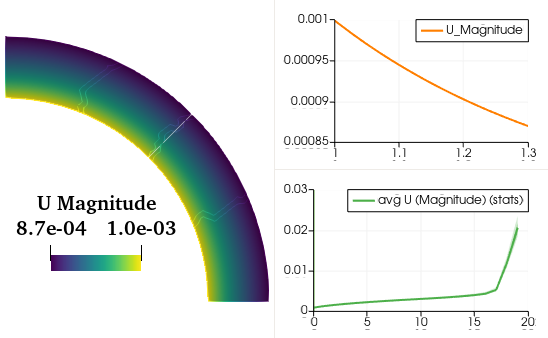
\includegraphics[width=0.45\textwidth]{./Images/test_psd_t0.png}}\hspace{1mm}\fbox{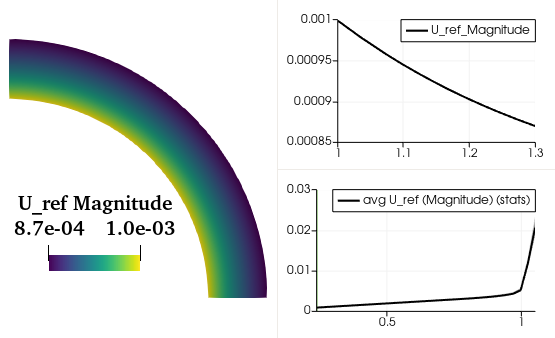
\includegraphics[width=0.456\textwidth]{./Images/test_fenics_t0.png}}\vspace{1mm}
\fbox{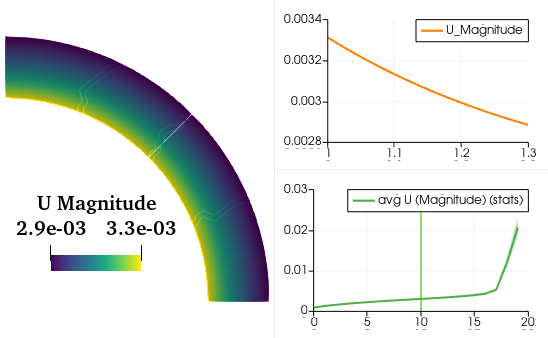
\includegraphics[width=0.45\textwidth]{./Images/test_psd_t10.png}}\hspace{1mm}\fbox{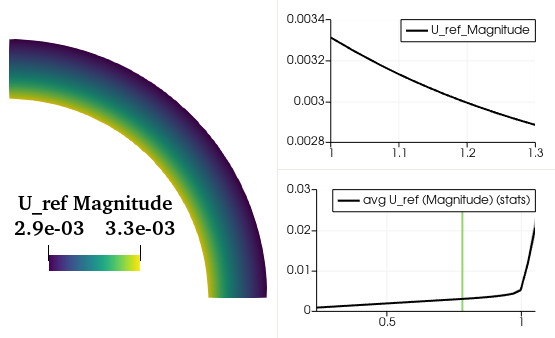
\includegraphics[width=0.456\textwidth]{./Images/test_fenics_t10.png}}\vspace{1mm}
\fbox{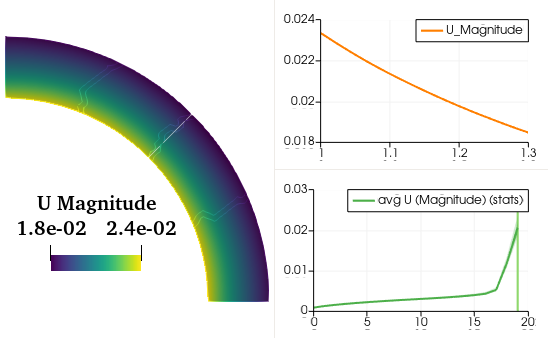
\includegraphics[width=0.45\textwidth]{./Images/test_psd_t19.png}}\hspace{1mm}\fbox{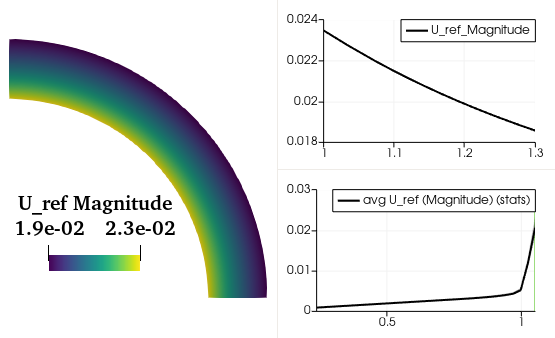
\includegraphics[width=0.456\textwidth]{./Images/test_fenics_t19.png}}\vspace{1mm}
\caption{Validation results comparison of PSD (left column) and reference code (right column) at different timesteps ($t_0, t_{10}, t_{19}$). Reference results used for comparison  were obtained by installing and running the FEniCS Solid Mechanics library [Garth N. Wells (2021)]. \label{comp2}}
\end{figure}

You are all done with your 2D elasto-plastic simulation with Mfront
interface.

\section{Validation}

To thoroughly validate PSD-MFront model and interface, the results
obtained from this tutorial can directly be compared to the ones
observed by (Garth N. Wells 2021). (Garth N. Wells 2021) present a
non-linear solid mechanics solver using the open-source FEniCS library.
Elasto-plastic von Mises material from the (Garth N. Wells 2021) solver
is compared in \cref{comp2,comp1,comp3}. The comparisons match with a
good order of accuracy.

\begin{figure}[h!] 
\centering
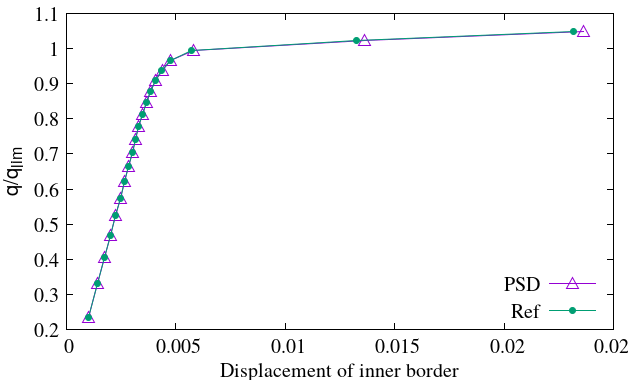
\includegraphics[width=0.45\textwidth]{./Images/final.png}
\caption{Validation of the displacement  movement of inner border movement obtained by PSD and another reference code.  Reference results used for comparison  were obtained by installing and running the FEniCS solid mechanics codes \url{https://bitbucket.org/fenics-apps/fenics-solid-mechanics}. \label{comp3}}
\end{figure}

\begin{figure}[h!]
\centering
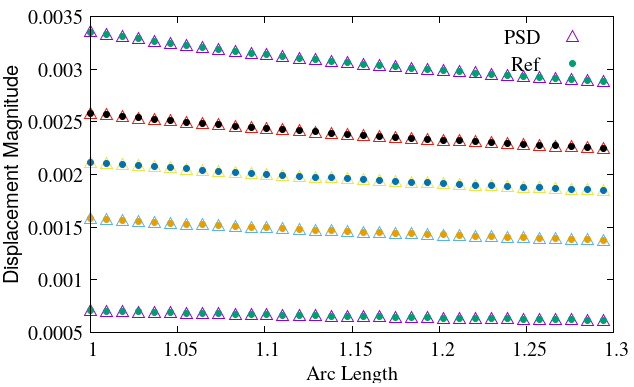
\includegraphics[width=0.45\textwidth]{./Images/t5.png}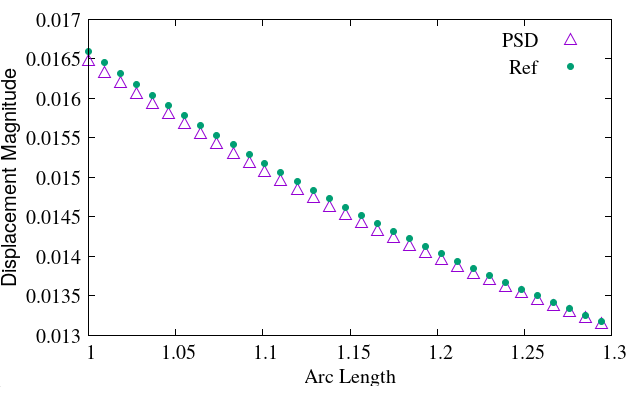
\includegraphics[width=0.45\textwidth]{./Images/t19.png}
\caption{Validation of the displacement field obtained by PSD and another reference code. The displacement magnitude is plotted on the central line which bisects the geometry into two. On the left time steps - $t_0,t_4,t_8,t_{12},t_{16}$ are plotted and on the right $t_{19}$. Reference results used for comparison  were obtained by installing and running the FEniCS Solid Mechanics library [Garth N. Wells (2021)]. \label{comp1}}
\end{figure}

\section*{Bibliography}\label{bibliography}
\addcontentsline{toc}{section}{Bibliography}

\hypertarget{refs}{}
\hypertarget{ref-Fenics}{}
Garth N. Wells, Kristian B. Ølgaard. 2021. ``FEniCS Solid Mechanics
library.''
\url{https://bitbucket.org/fenics-apps/fenics-solid-mechanics/src/master/}.
